%%%%%%%%%%%%%%%%%%%%%%%%%%%%%%%%%%%%%%%%%%%%%%%%%%%%%%%
%               File: OSAtemp.tex                     %
%                VERSION: 3.1                         %
%              Date: May 28, 2004                     %
%                                                     %
%    LaTeX template file for use with OSA journals    %
%         JOSA A, JOSA B, Applied Optics, and         %
%                   Optics Letters                    %
%                                                     %
%   This file requires the substyle file osajnl.rtx,  %
%       running under REVTeX 4.0 and LaTeX 2e,        %
%                           or                        %
%   the style file osajnl.sty, running under LaTeX 2e %
%                                                     %
%       USE THE FOLLOWING REVTEX 4.0 OPTIONS:         %
%  \documentclass[osajnl,preprint,showpacs]{revtex4}  %
%                                                     %
%         USE THE FOLLOWING LaTeX OPTIONS:            %
%           \documentclass[11pt]{article}             %
%           \usepackage{osajnl}                       %
%                                                     %
%                                                     %
%      NOTE: LaTeX 2.09 IS NO LONGER SUPPORTED        %
%                                                     %
%      (C) 2004 The Optical Society of America        %
%                                                     %
%%%%%%%%%%%%%%%%%%%%%%%%%%%%%%%%%%%%%%%%%%%%%%%%%%%%%%%

% \documentclass[osajnl,preprint,showpacs]{revtex4}  %% REVTeX 4.0
%
%%%%%%%%%%%%%%%%%%%%%%%%%%%%%%%%%%%%%%%%%%%%%%%%%%%%%%%%%%%%%%%%%
%% Delete any REVTeX output files before running in LaTeX mode
%%%%%%%%%%%%%%%%%%%%%%%%%%%%%%%%%%%%%%%%%%%%%%%%%%%%%%%%%%%%%%%%%

\documentclass[12pt,letterpaper]{article}          %% LaTeX 2e (preferred)
\usepackage{osajnl}
\usepackage[draft]{hyperref} % optional

\begin{document}

\title{Template for manuscript submissions to \emph{Applied Optics}, JOSA A, JOSA B, and \emph{Optics Letters}}

\author{John Q. Author}
%% for REVTeX4, each author name can be set in a separate \author{} field

\address{Publications Department, Optical Society of America,
\\  2010 Massachusetts Avenue, N.W., Washington, D.C. 20036}

\email{jqaut@osa.org}

\begin{abstract}The abstract should be less than 100 words. 
Detailed instructions on manuscript preparation are available in the document \texttt{OSAstyle.tex},  and additional information on manuscript
preparation and submission is available on the home page for each
OSA journal; see \mbox{\href{http://www.opticsinfobase.org}{http://www.opticsinfobase.org}}.
\end{abstract}

\ocis{000.0000, 999.9999.}% REPLACE WITH CORRECT OCIS CODES FOR YOUR ARTICLE
                          % NOTE: \ocis{} IS ALIASED TO \pacs{} BUT MUST
                          % FORMAT THE TERMS CORRECTLY FOR EACH JOURNAL

\maketitle %% NULL FUNCTION WITH LATEX 2e; required for REVTeX4

\section{Introduction}
Refer to \texttt{OSAstyle.tex} for guidelines on manuscript preparation, use of \mbox{Bib\TeX}, and similar. Our new style file (July 2003 version of \texttt{osajnl.sty}) has reduced line space to help save paper.

To facilitate conversion, place all math in a proper math environment. For example, expression $3\times 4 = 12$ should be set this way, \texttt{\$3$\backslash$times 4=12\$}, not this way, \texttt{3 \$$\backslash$times\$4=12}.
\section{Conclusion}

After the manuscript is proofread, the {\tt .tex} file and figures
should be archived with tar-gzip compression. Do not include
subdirectories within the archive.

To upload your manuscript, follow the instructions on the each
journal's homepage (see \mbox{\href{http://www.opticsinfobase.org}{http://www.opticsinfobase.org}}).
Authors should feel free to contact OSA staff for assistance; details are available at \href{InfoBase}{http://www.opticsinfobase.org}.

%\appendix

%\section*{Appendix A: Sample}
%\setcounter{equation}{0}
%\renewcommand{\theequation}{A{\arabic{equation}}}

%\begin{equation}
%a+b=c.
%\end{equation}


\begin{thebibliography}{99}
%%Do not include separate BibTeX files; if BibTeX is used,
%% paste the output (contents of .bbl file) here.

\bibitem{1} ...

\bibitem{2} ...

\end{thebibliography}

\newpage

\section*{List of Figure Captions}

Fig. 1. Multipanel figure assembled into one file with proper
arrangement and labeling.
%\noindent Fig. 2. ...

%\noindent Fig. 3. ...


\newpage
%% sample figure environment
  \begin{figure}[htbp]
  \centering
  \includegraphics[width=8.3cm]{OT10000F1.eps}
  \caption{Multipanel figure assembled into one EPS file with proper arrangement and labeling. AO10000F1.eps.}
  %% \label{}
  \end{figure}


\end{document}
